\documentclass[a6paper,11pt]{article}
%\usepackage[T1]{fontenc}
\usepackage[british]{babel}
\usepackage[utf8]{inputenc}
\usepackage{float, graphicx,amsmath,amsfonts,cite,enumerate}
\usepackage[final]{pdfpages}
\usepackage{wrapfig}
\usepackage[margin=0.3in]{geometry}
\usepackage{sidspaltHack}

\newcommand{\mel}[1]{\small\textbf{\textit{mel. #1 \\}}}


\setlength{\oddsidemargin}{-0.47in}
\setlength{\textwidth}{235pt}

\pagestyle{empty}

\begin{document}
\nysida{16}{1}
\huge$\Omega\omega$ Noter\\
\vspace{-20pt}
\begin{center}
\Large$\omega1$. Du gamla du fria
\end{center}
\vspace{-40pt}
\begin{figure}[!h]
\hspace{-10pt}
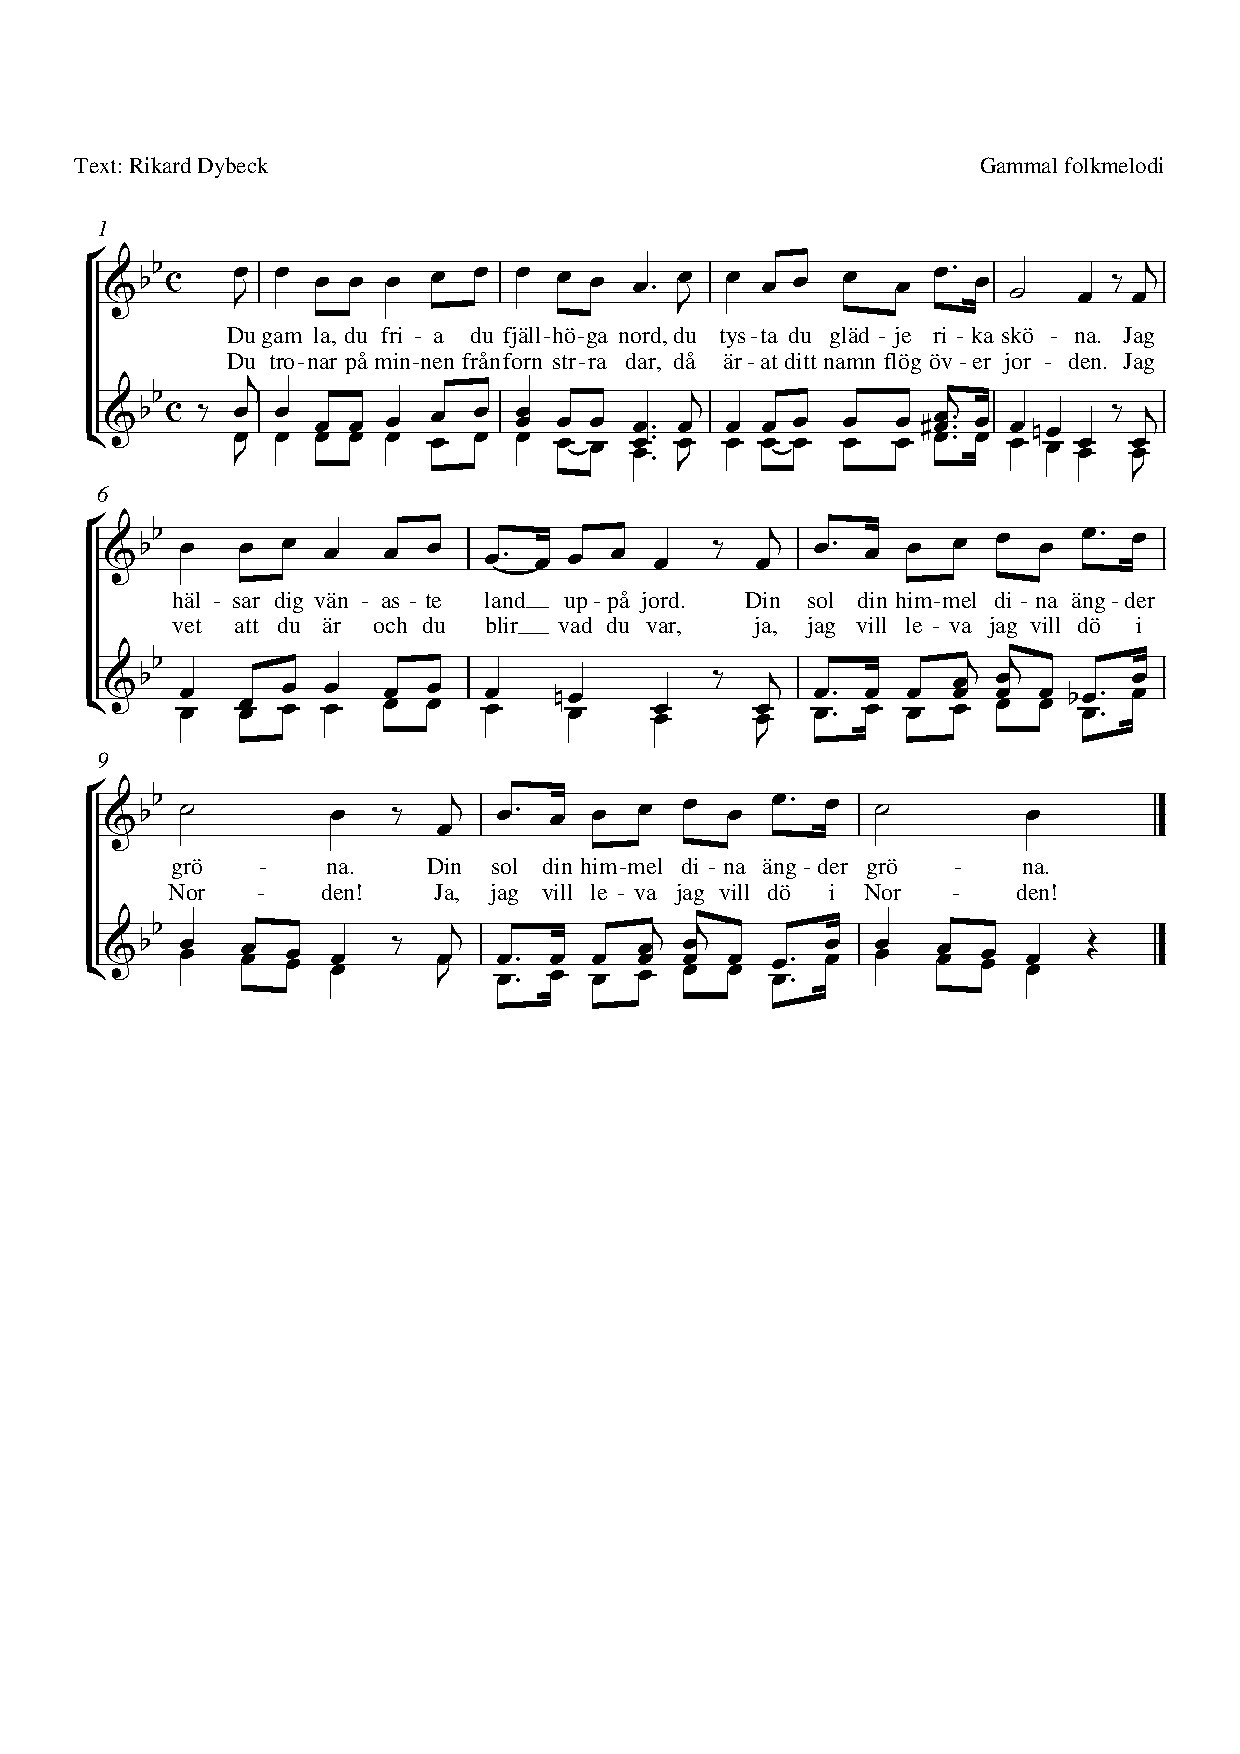
\includegraphics[width=\textwidth]{du_gamla_du_fria}
\end{figure}

\nysida{16}{2}
\setlength{\oddsidemargin}{-0.67in}
\begin{center}
\Large$\omega2$. Kungssången
\end{center}
\vspace{-40pt}
\begin{figure}[!h]
\centering
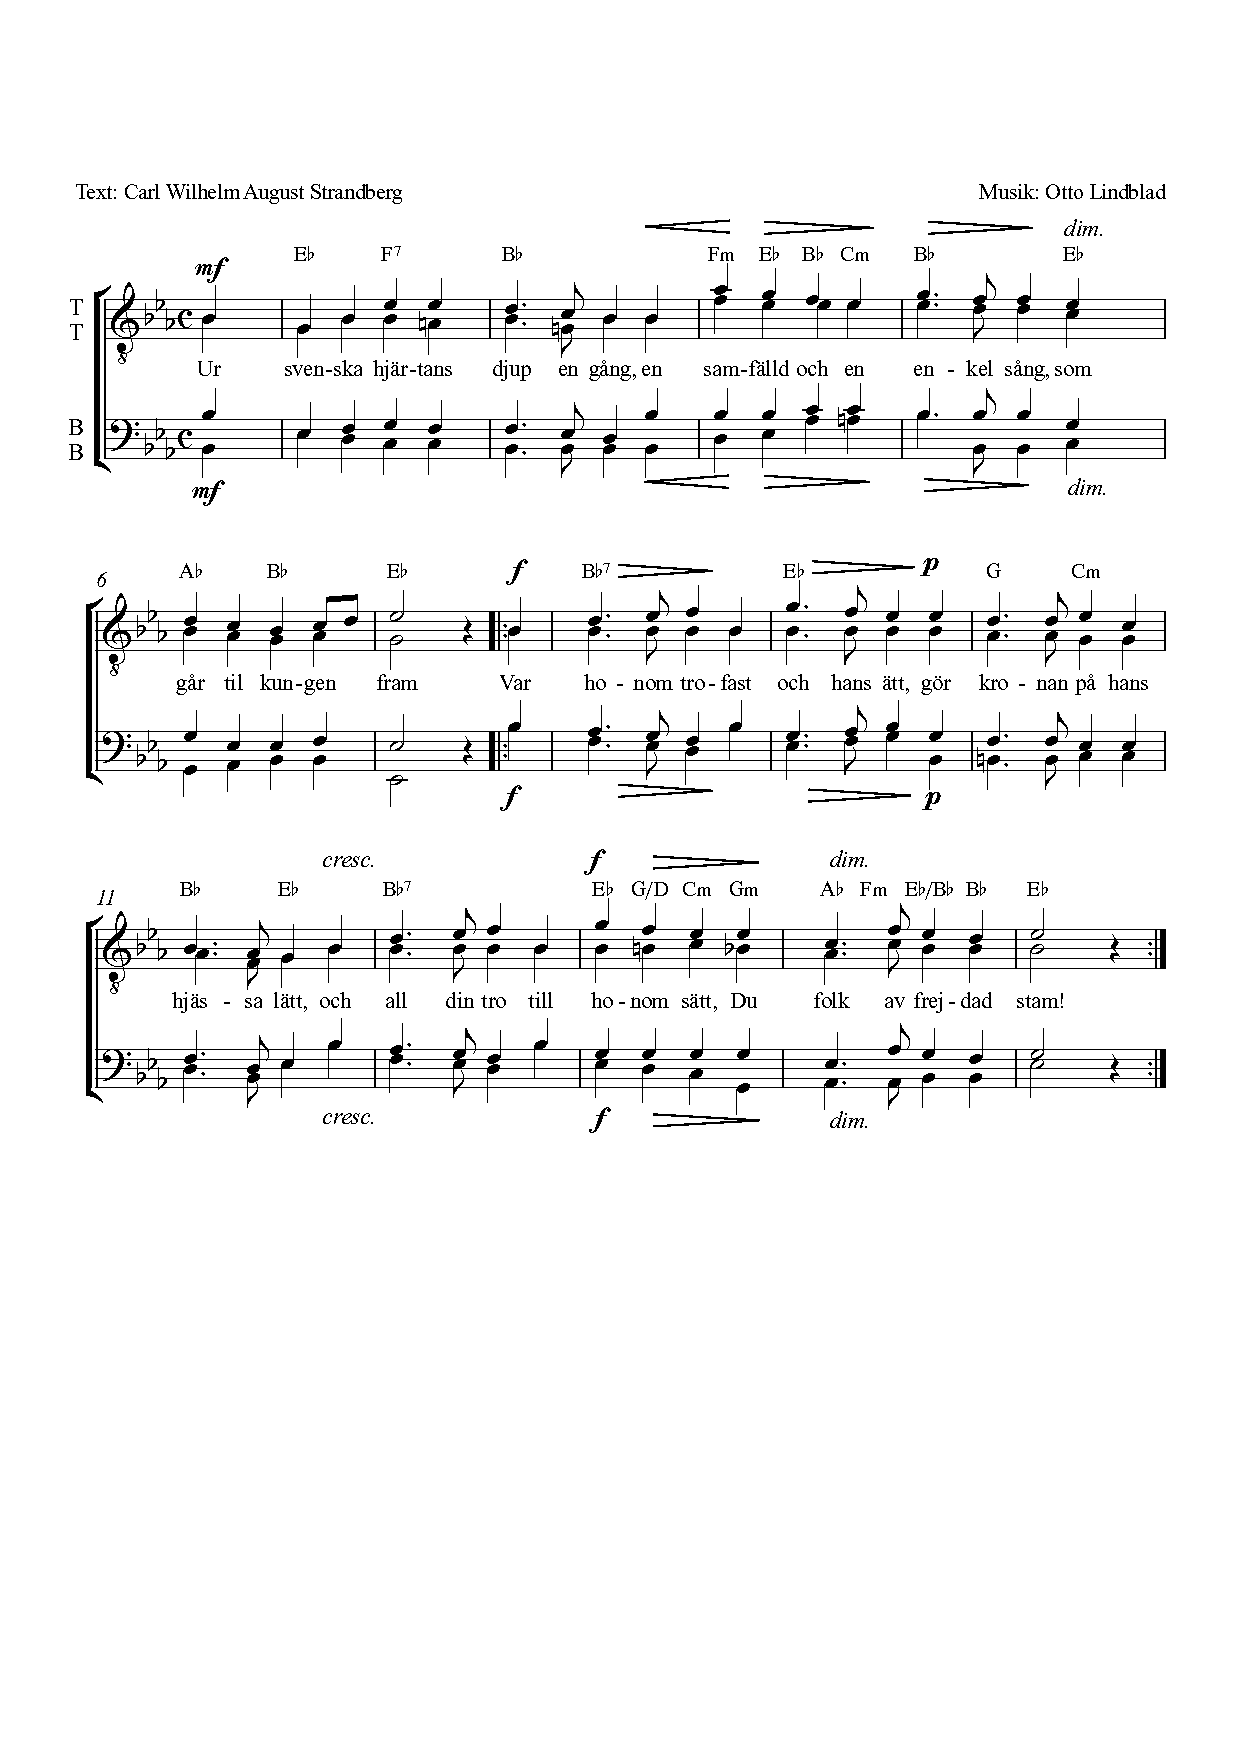
\includegraphics[width=\textwidth]{kungssangen}
\end{figure}

\nysida{16}{3}
\setlength{\oddsidemargin}{-0.47in}
\begin{center}
\Large$\omega 3$. Sveriges flagga
\end{center}
\vspace{-40pt}
\begin{figure}[!h]
\centering
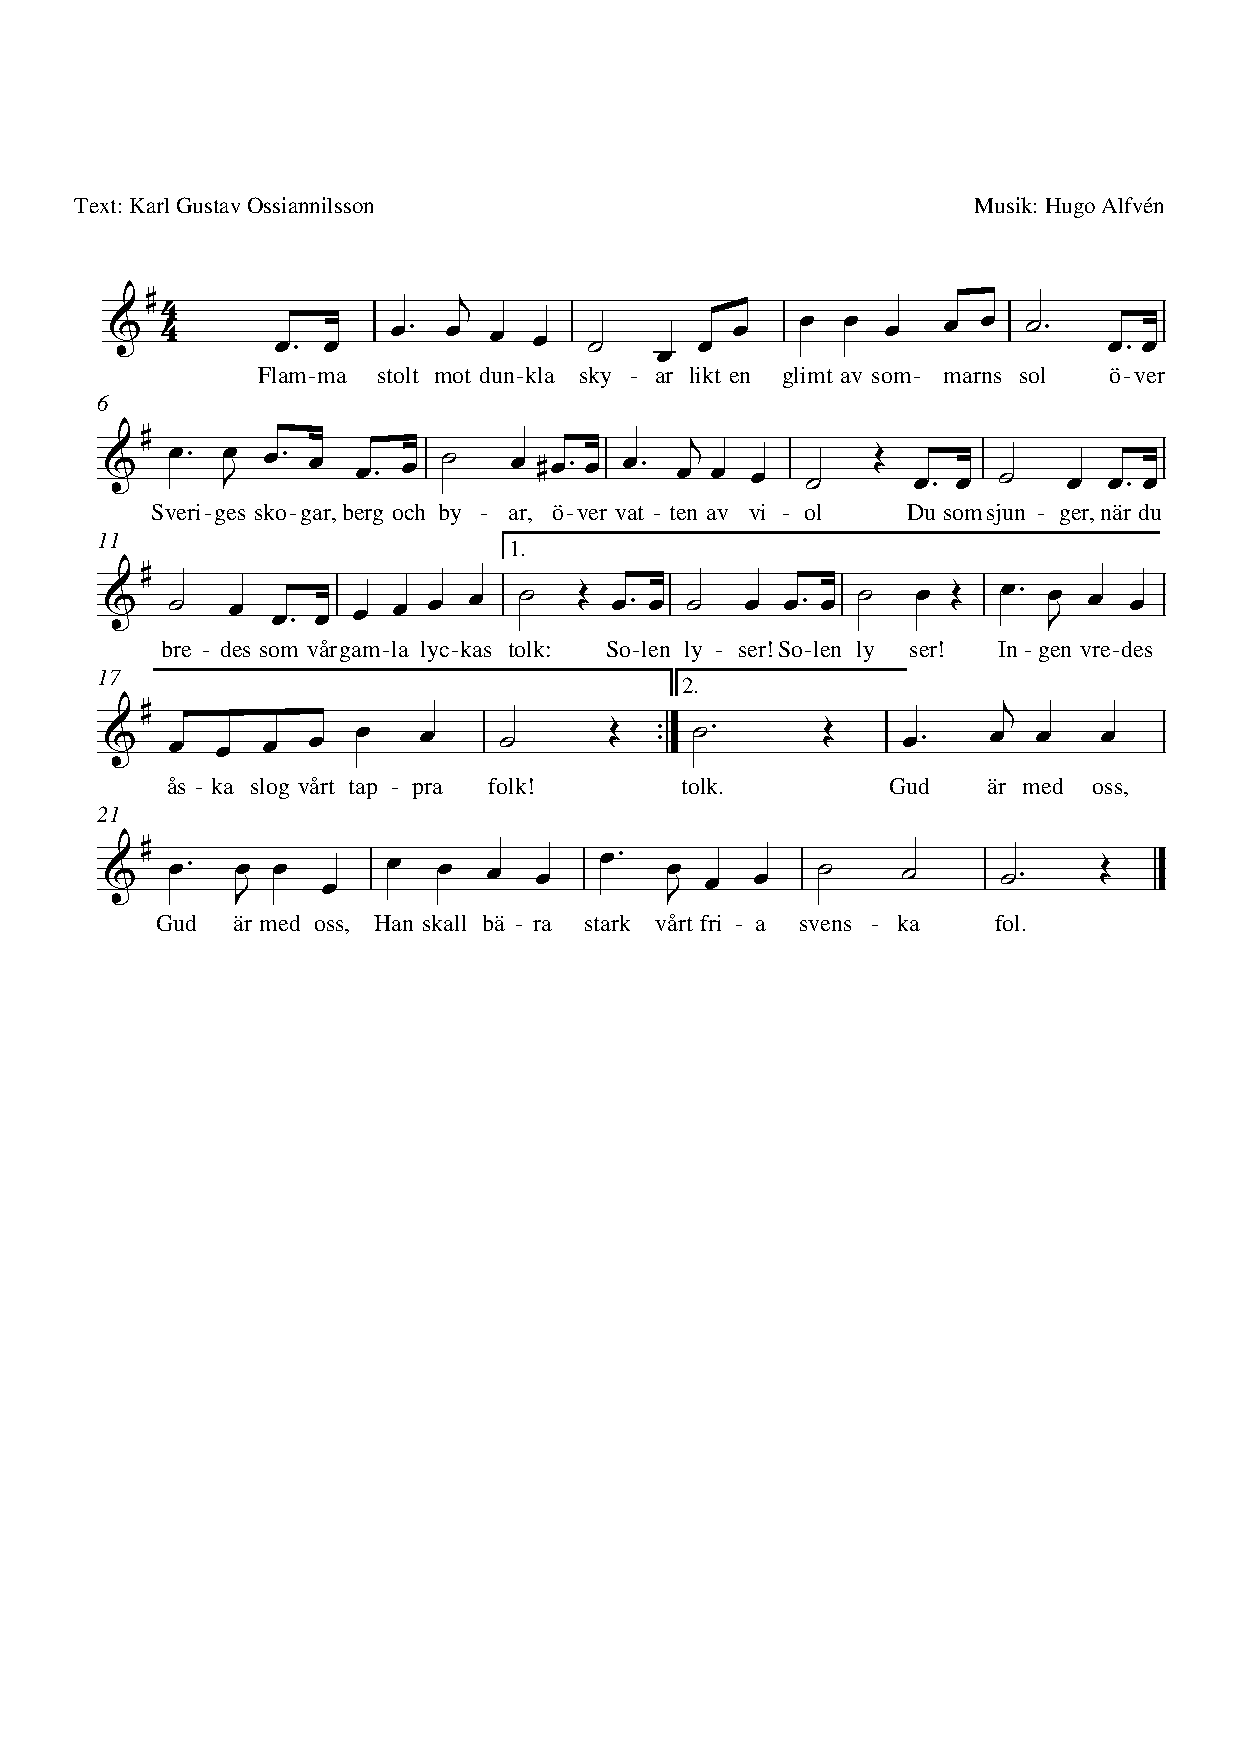
\includegraphics[width=\textwidth]{sveriges-flagga}
\end{figure}

\nysida{16}{4}
\setlength{\oddsidemargin}{-0.67in}
\begin{center}
\Large$\omega4$. Porthos visa
\end{center}
\vspace{-40pt}
\begin{figure}[!h]
\centering
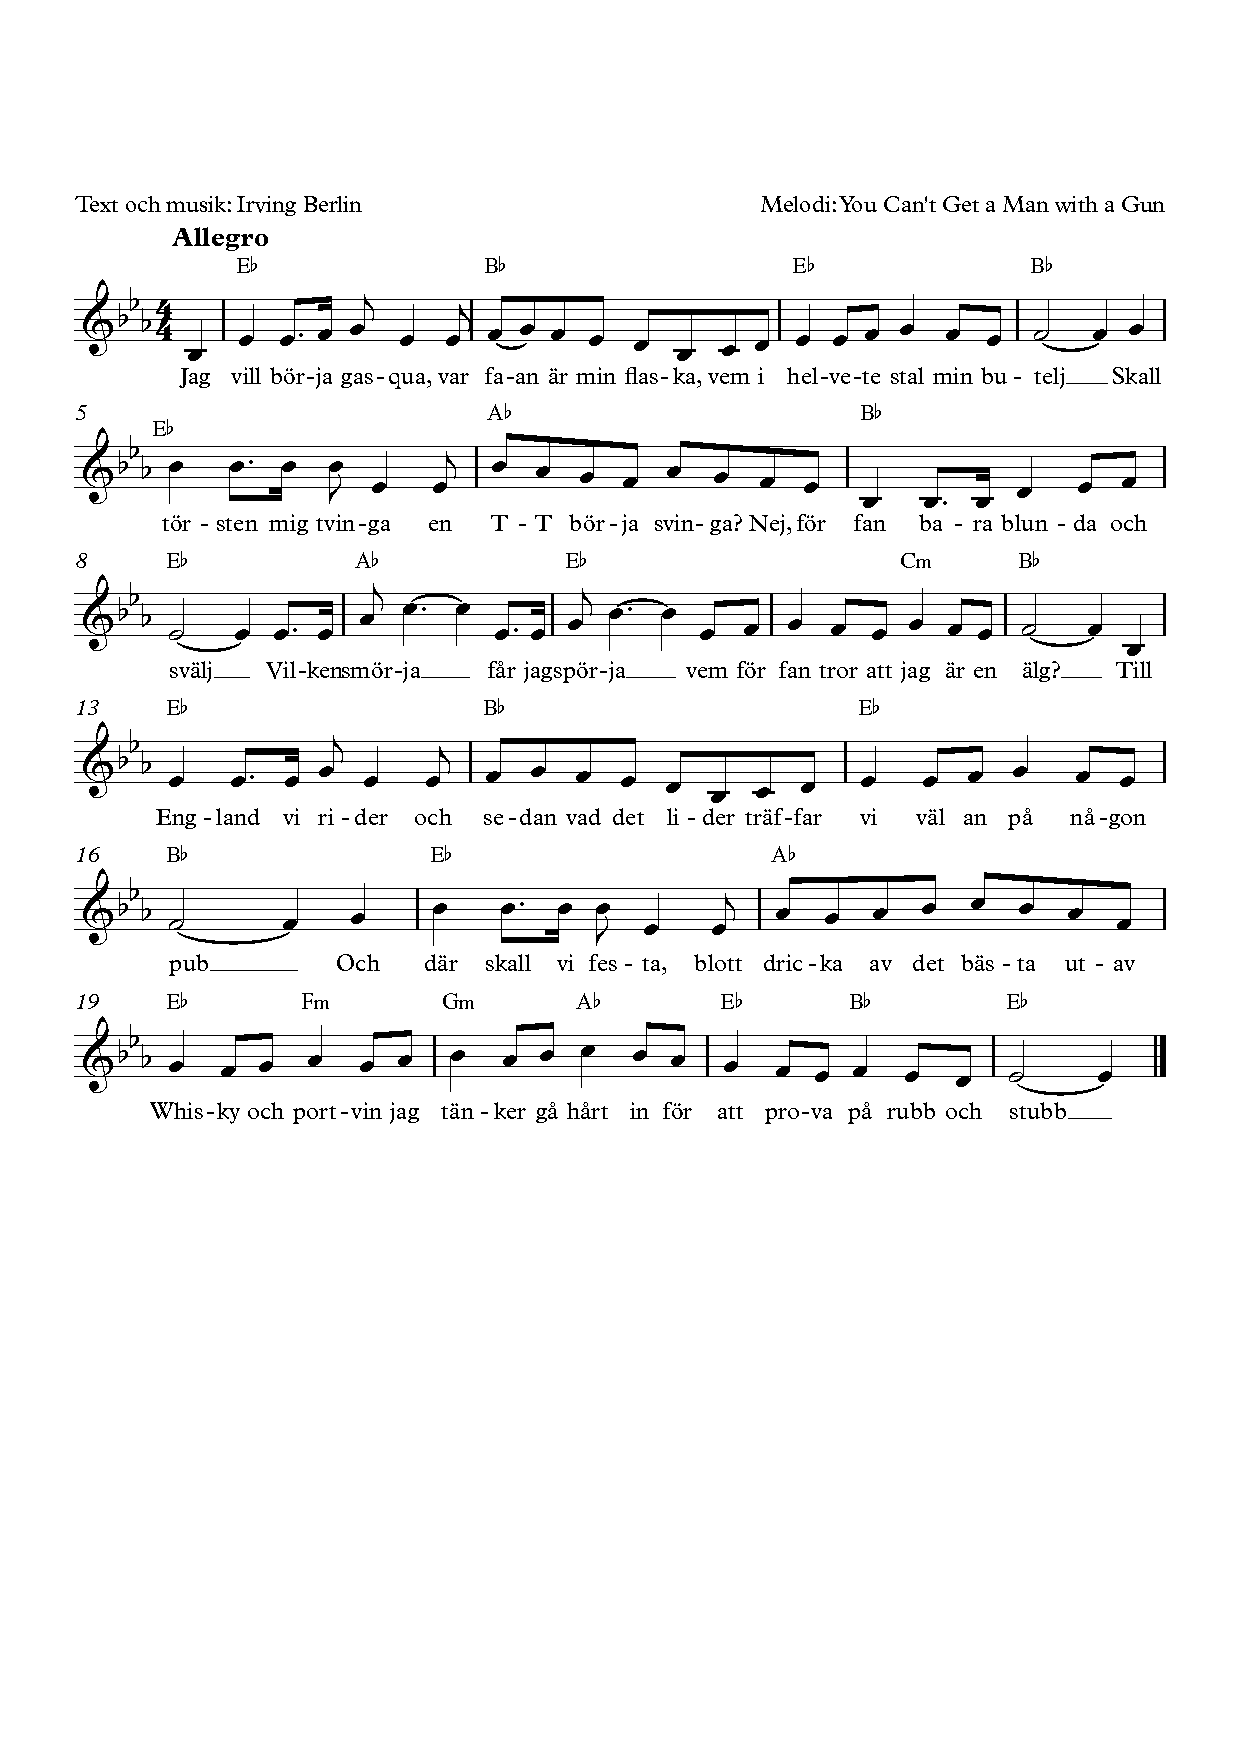
\includegraphics[width=\textwidth]{porthos}
\end{figure}

\nysida{16}{5}
\setlength{\oddsidemargin}{-0.47in}
\begin{center}
\Large$\omega5$. Lyft ditt välförsedda glas
\end{center}
\vspace{-40pt}
\begin{figure}[!h]
\centering
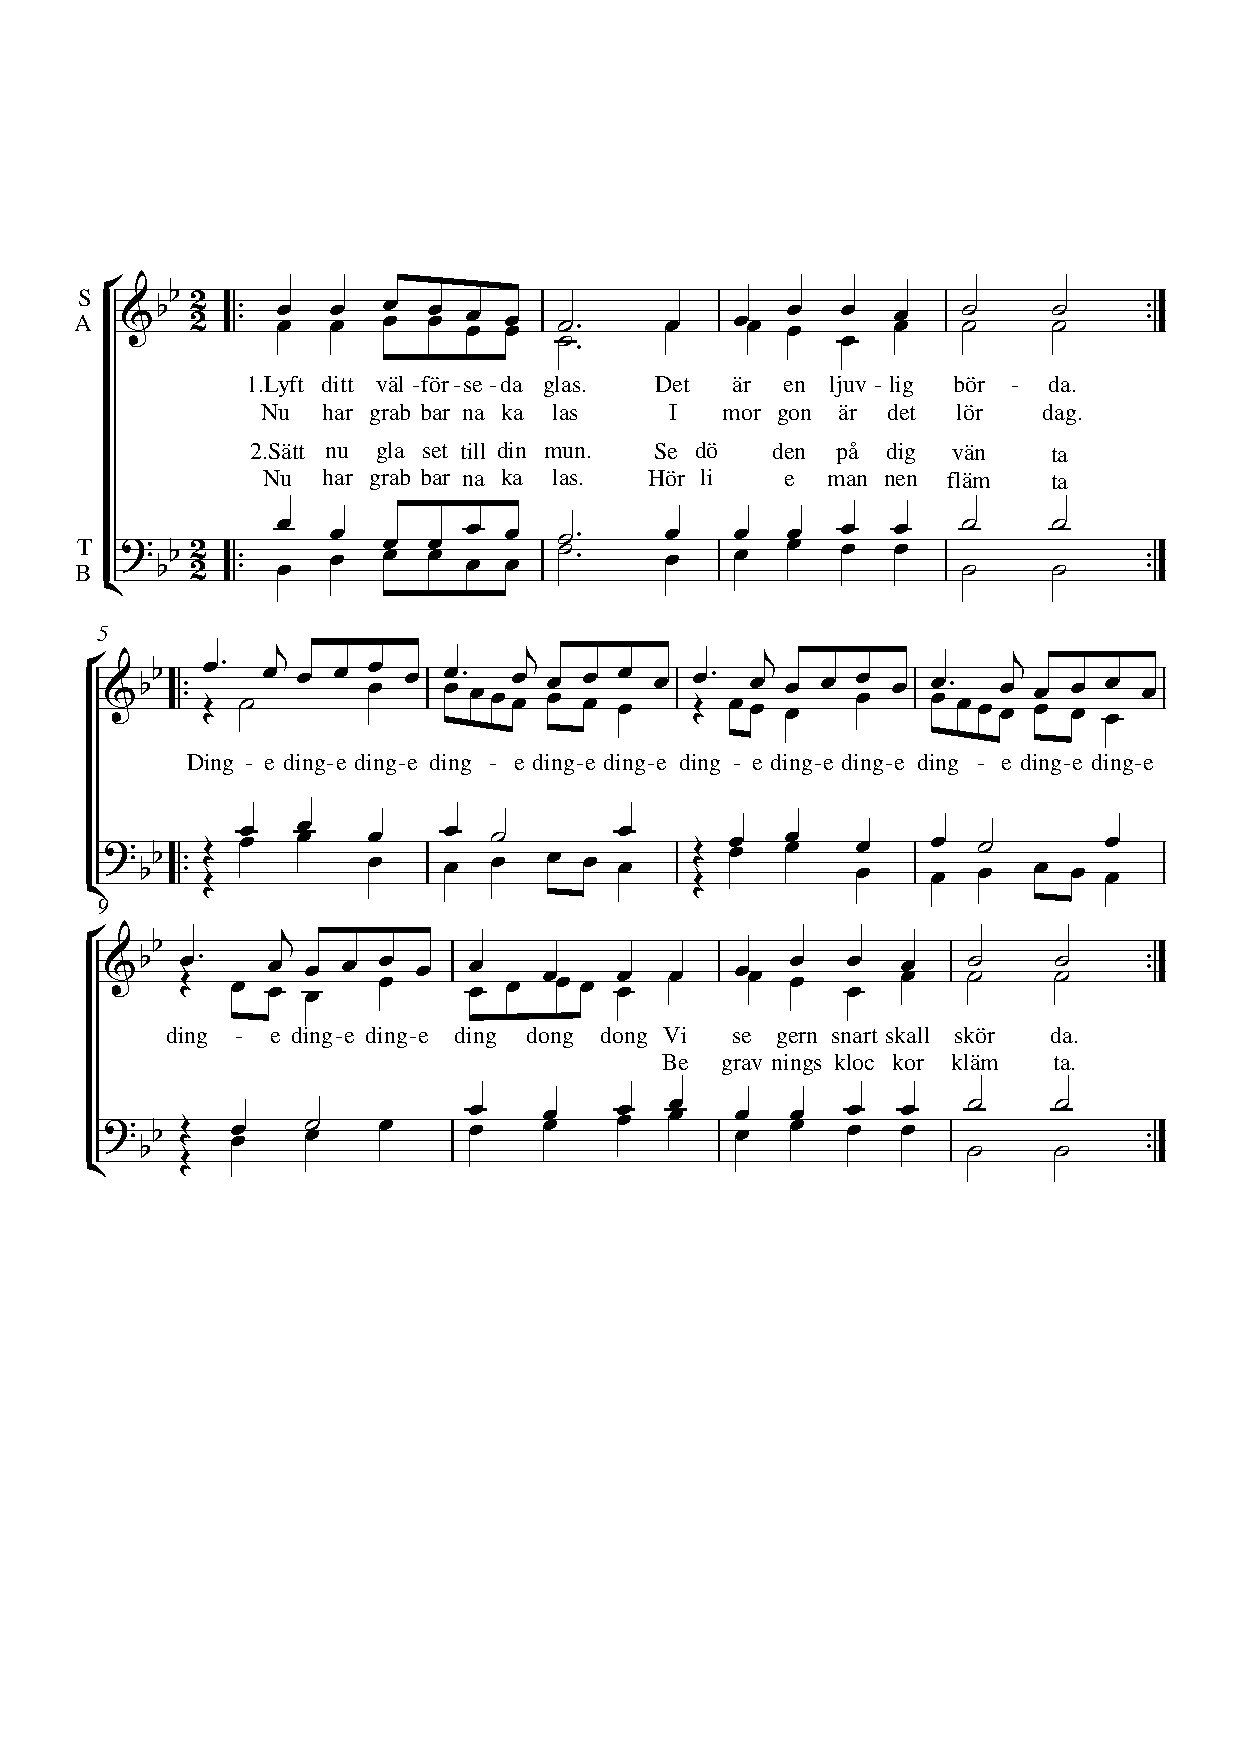
\includegraphics[width=\textwidth]{lyft-ditt-valforsedda}
\end{figure}

\nysida{16}{6}
\setlength{\oddsidemargin}{-0.67in}
\begin{center}
\Large$\omega6$. Längtan till landet
\end{center}
\vspace{-40pt}
\begin{figure}[!h]
\centering
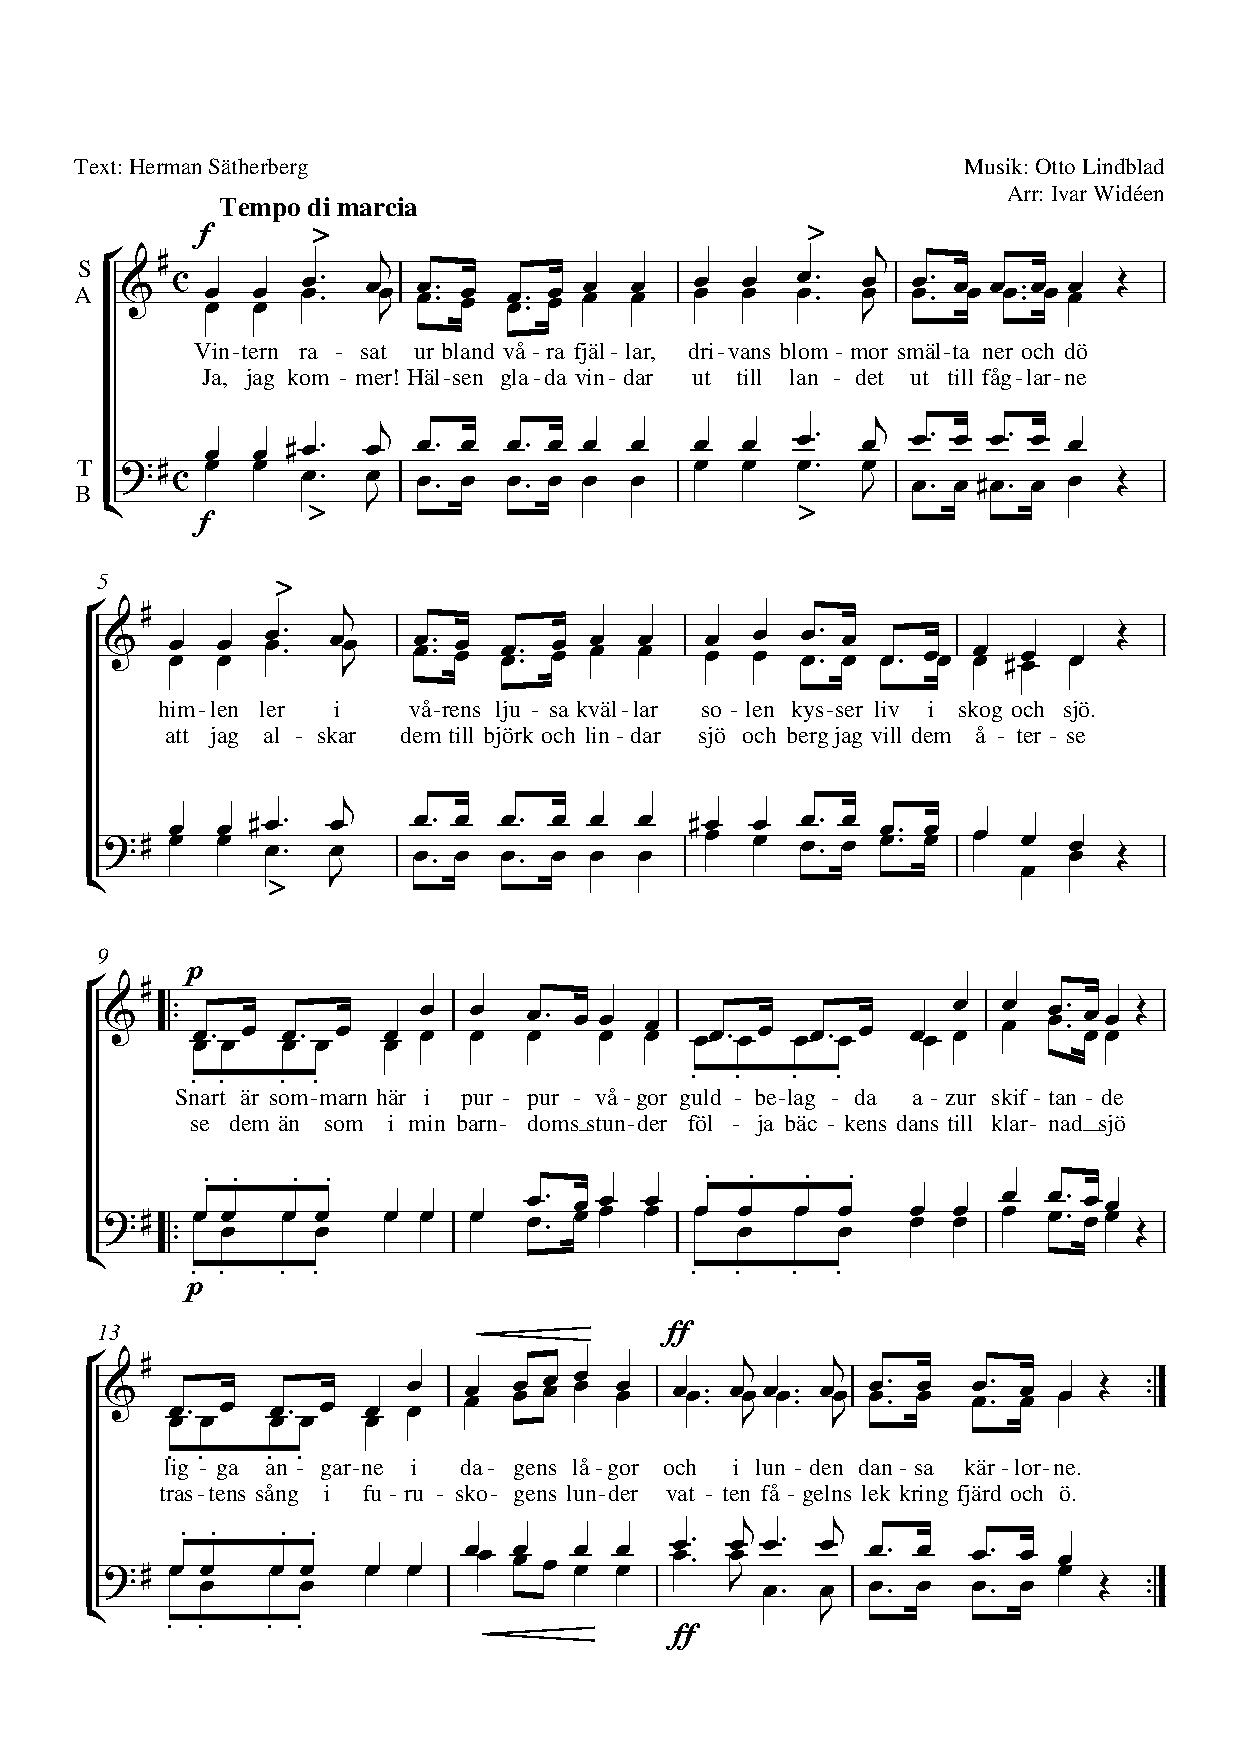
\includegraphics[width=\textwidth]{langtan-till-landet}
\end{figure}

\nysida{16}{7}
\setlength{\oddsidemargin}{-0.47in}
\begin{center}
\Large$\omega7$. Amanda Lundbom
\end{center}
\vspace{-40pt}
\begin{figure}[!h]
\centering
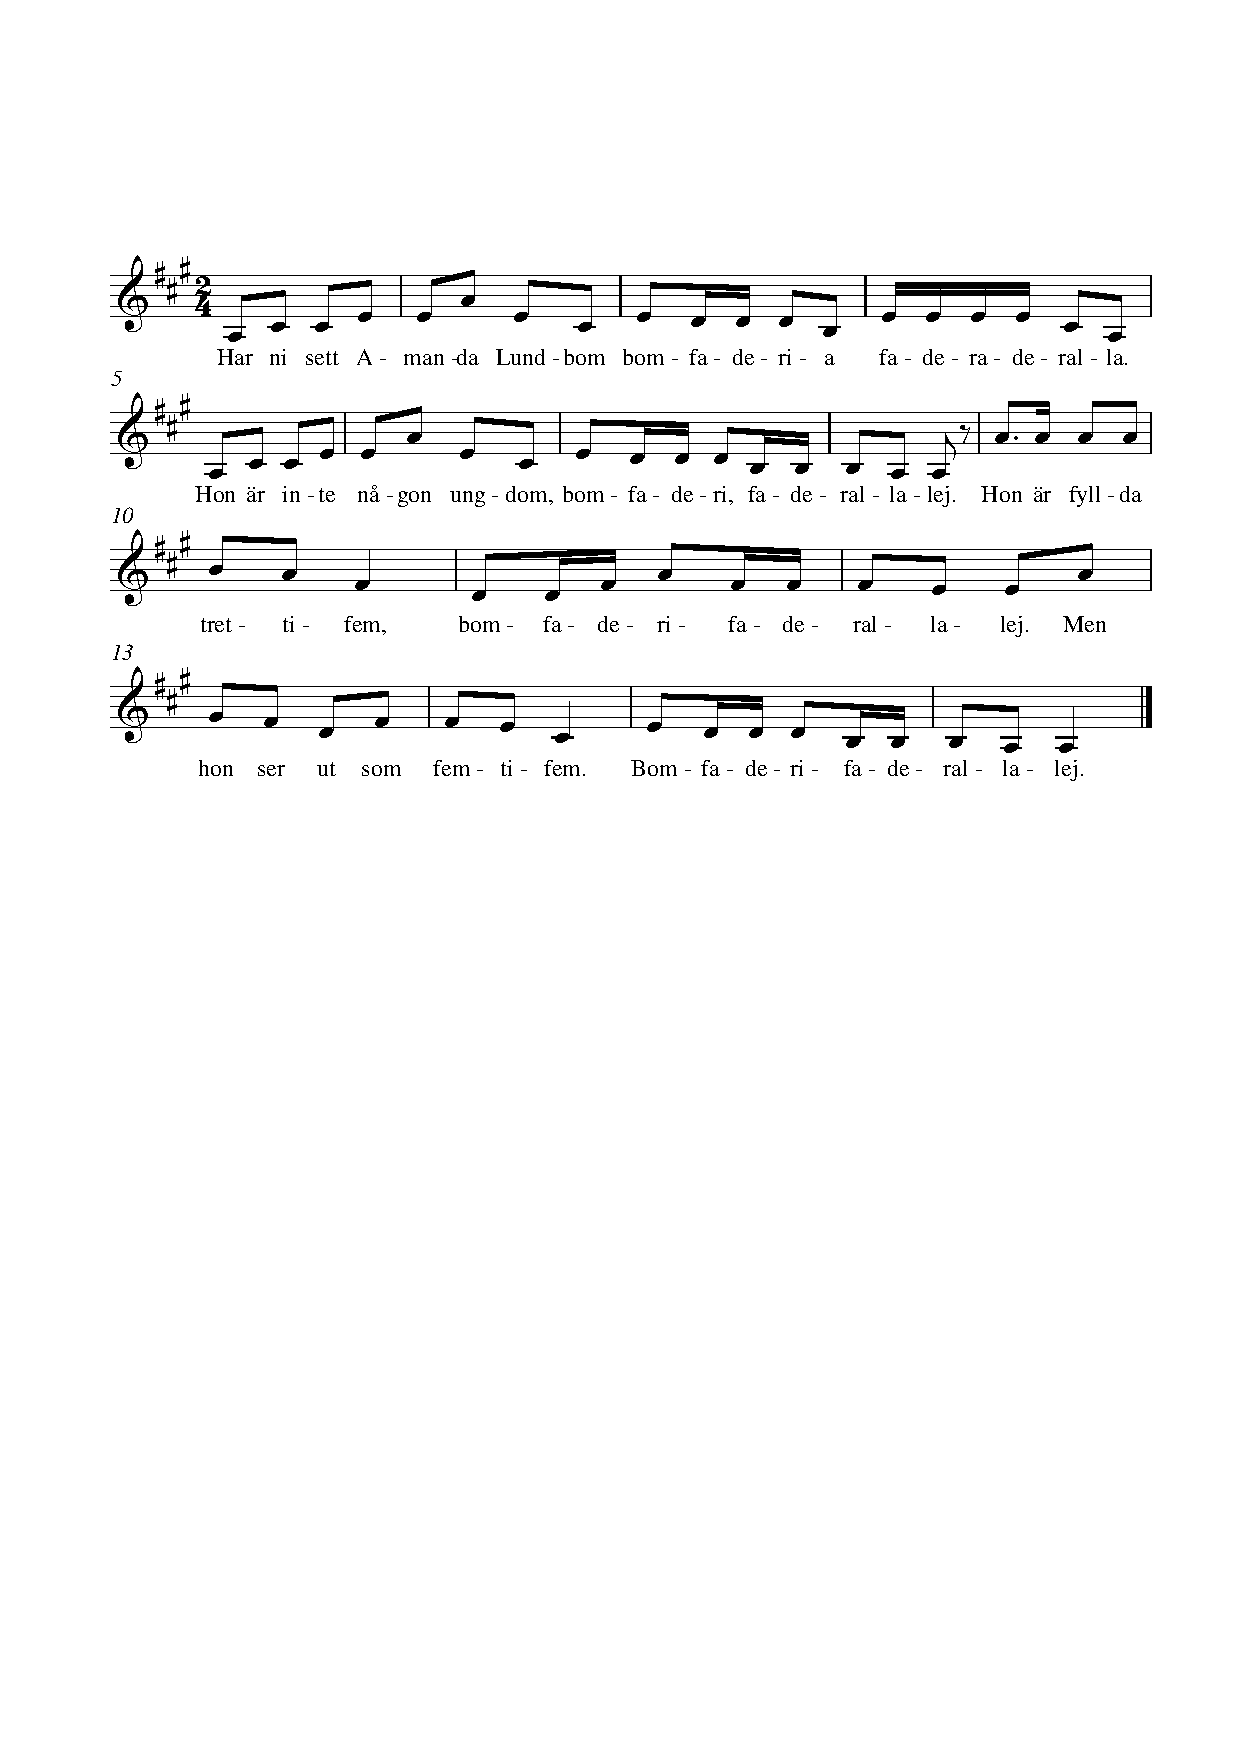
\includegraphics[width=\textwidth]{amandalundbom}
\end{figure}

\nysida{16}{8}
\setlength{\oddsidemargin}{-0.67in}
\begin{center}
\Large$\omega8$. Smedsvisa
\end{center}
\vspace{-40pt}
\begin{figure}[!h]
\centering
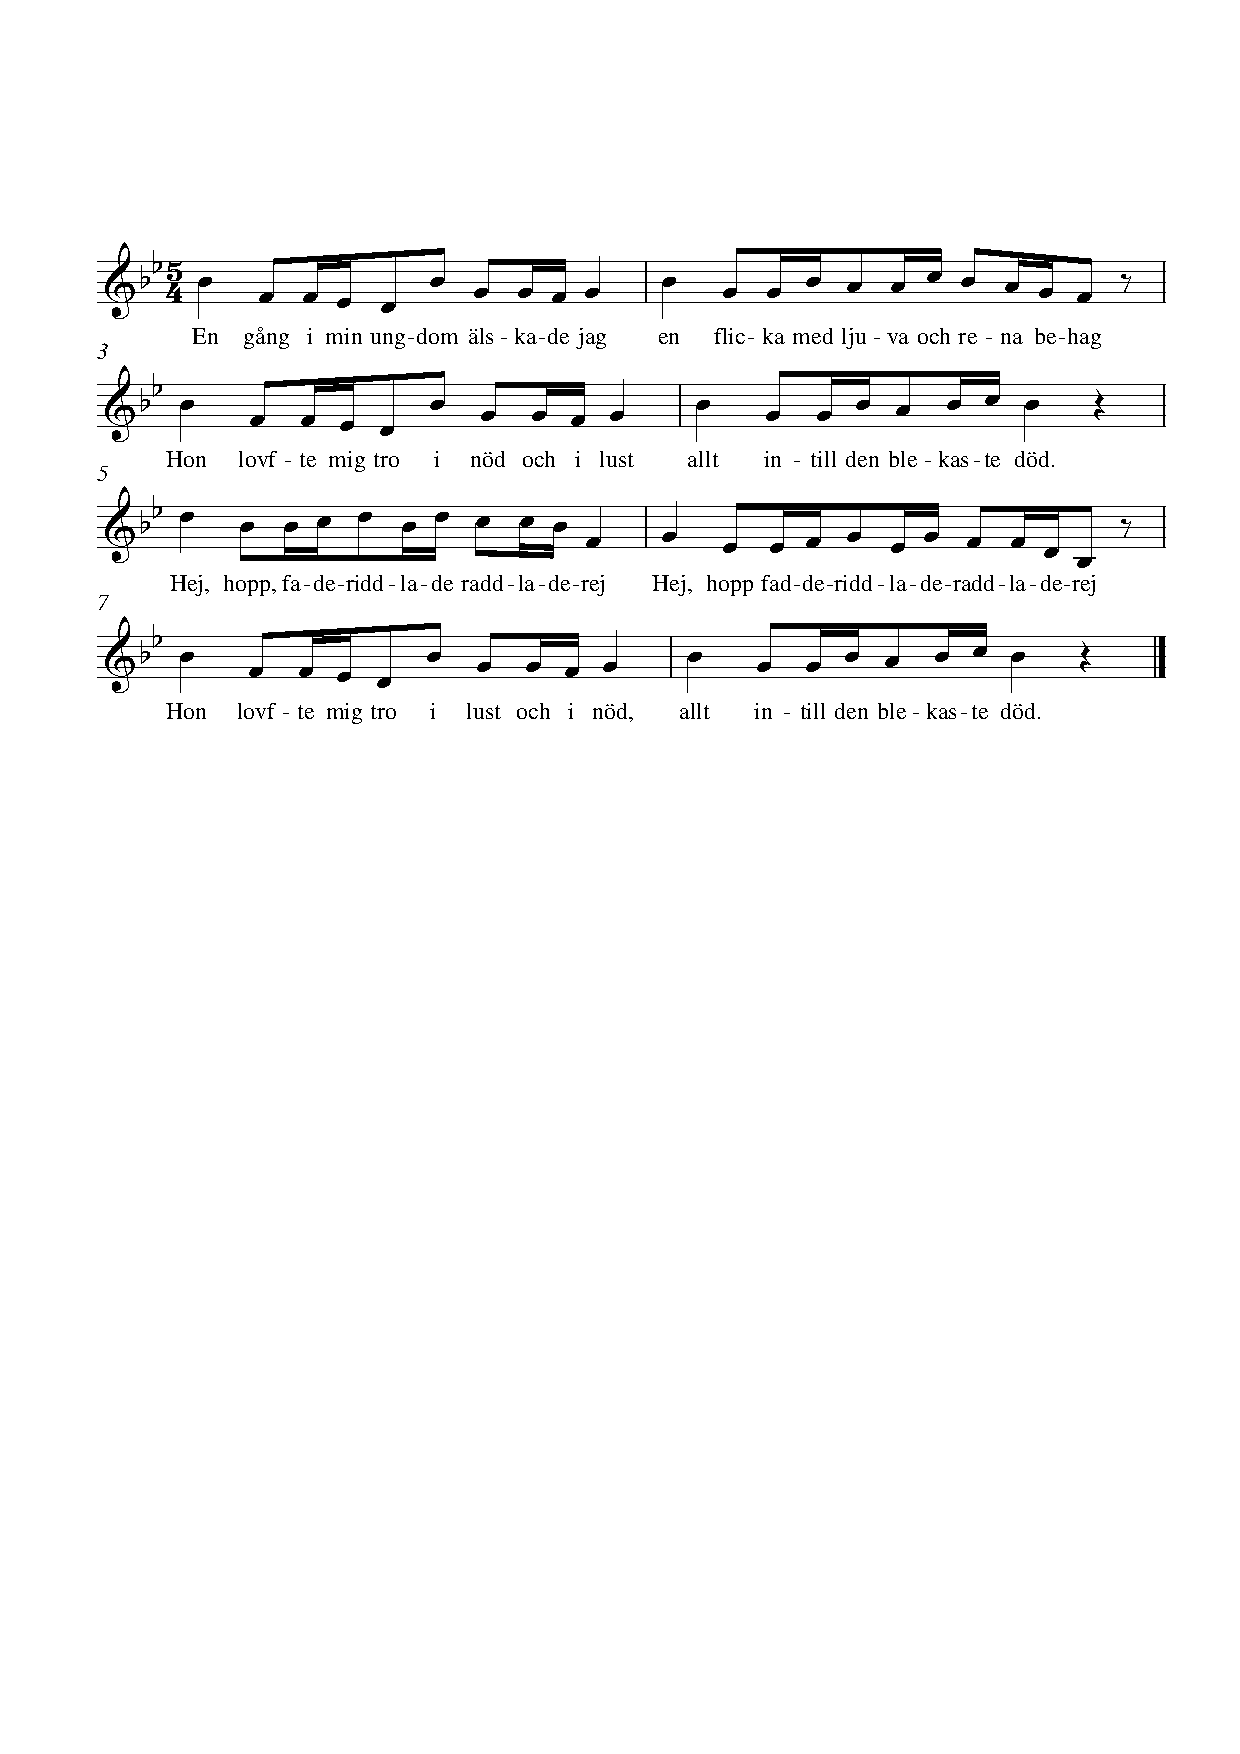
\includegraphics[width=\textwidth]{smedsvisa}
\end{figure}

\nysida{16}{9}
\setlength{\oddsidemargin}{-0.47in}
\begin{center}
\Large$\omega9$. Molltoner från Norrland
\end{center}
\vspace{-40pt}
\begin{figure}[!h]
\centering
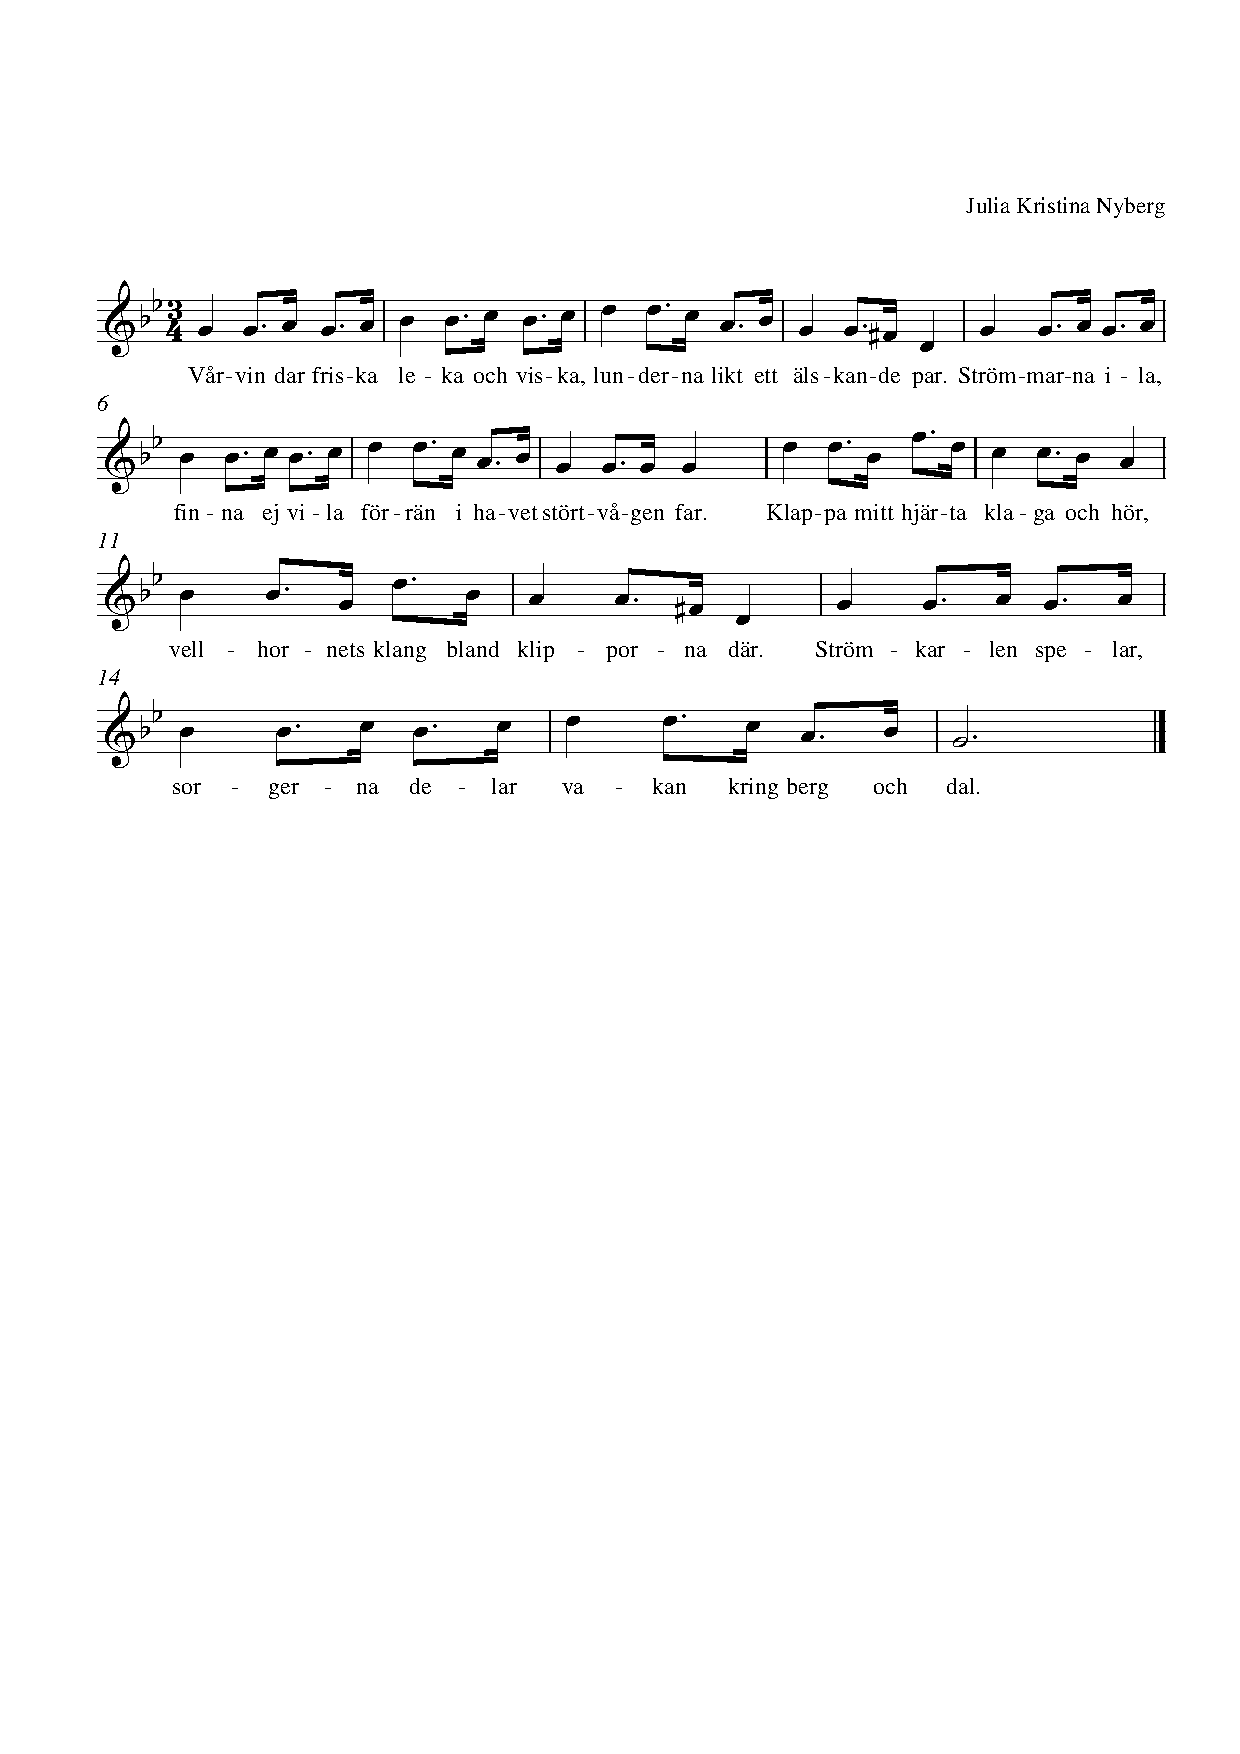
\includegraphics[width=\textwidth]{molltoner}
\end{figure}

\nysida{16}{10}
\setlength{\oddsidemargin}{-0.67in}
\begin{center}
\Large$\omega10$. Nu grönskar det
\end{center}
\vspace{-40pt}
\begin{figure}[!h]
\centering
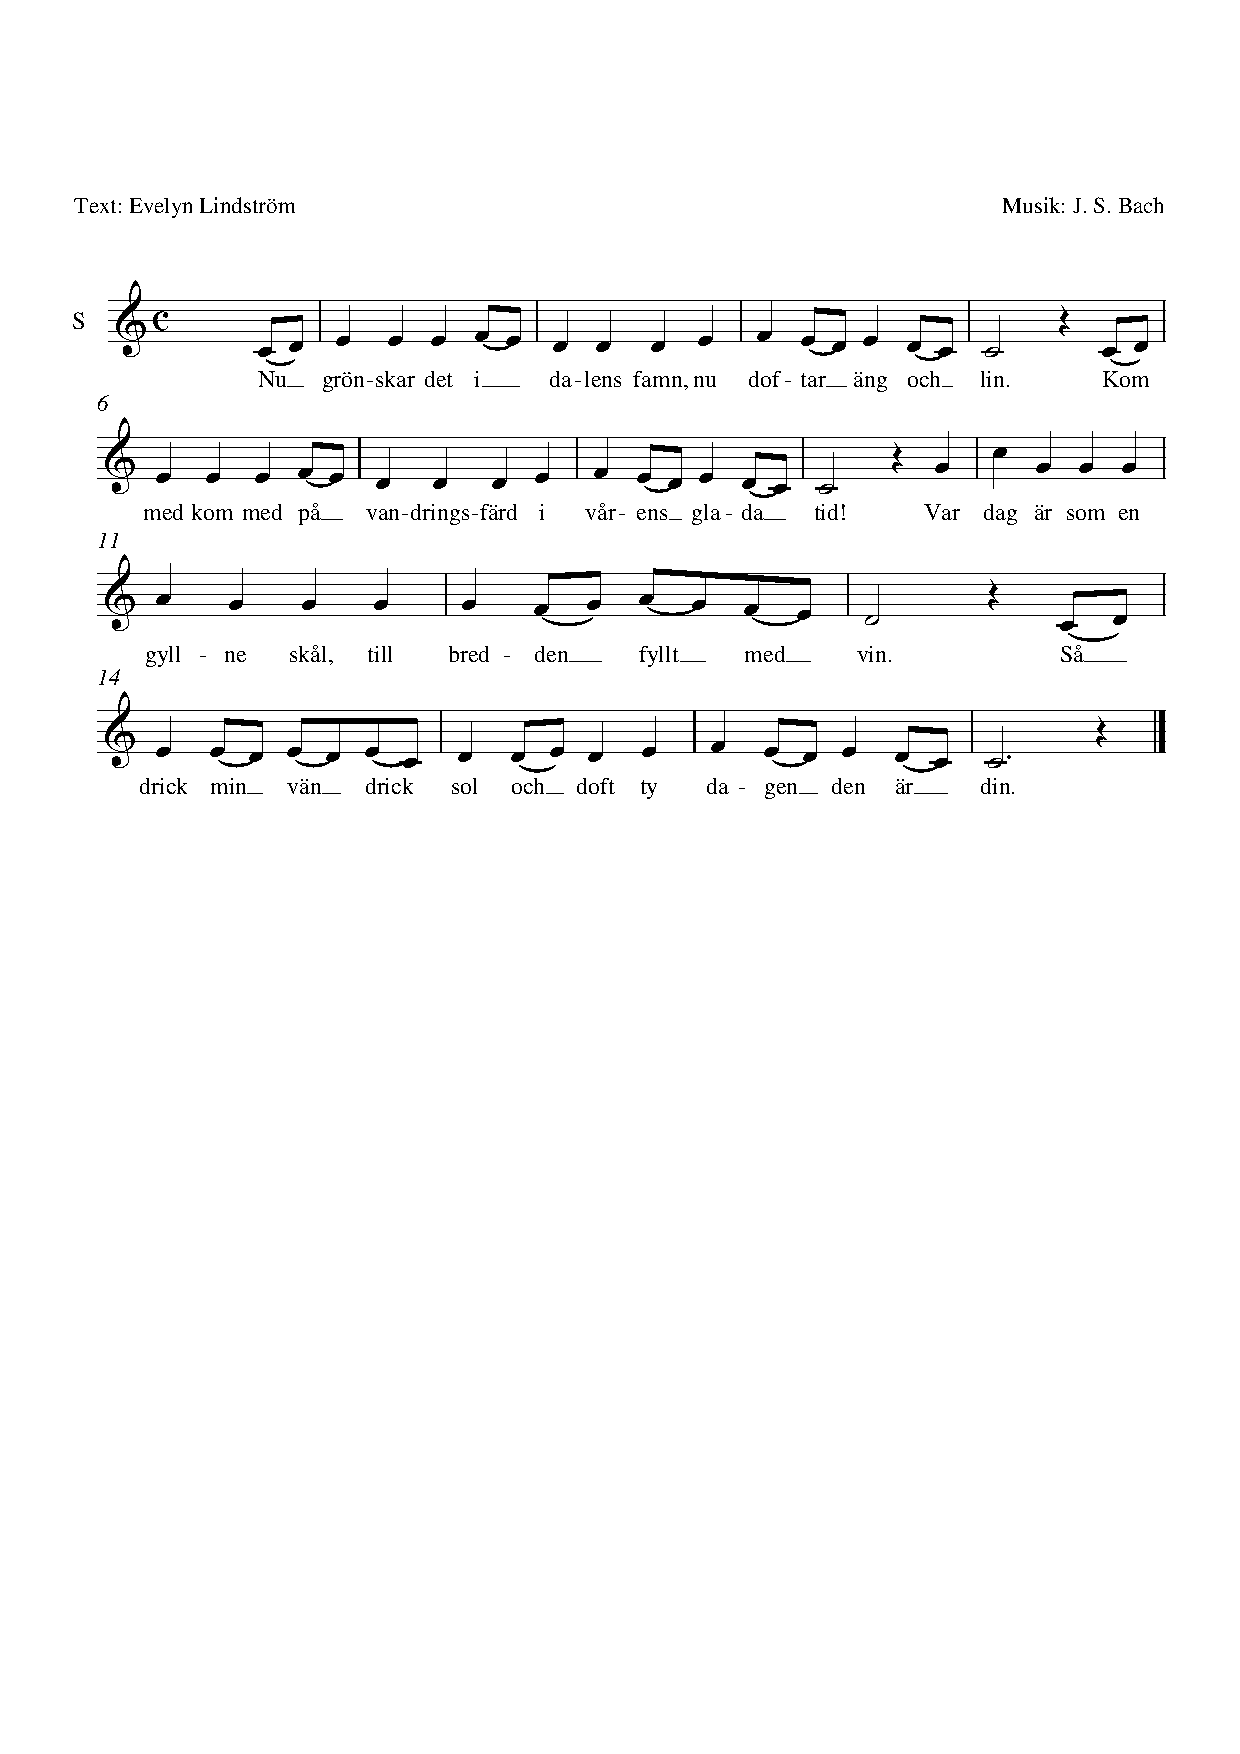
\includegraphics[width=\textwidth]{nugronskardet}
\end{figure}

\nysida{16}{11}
\setlength{\oddsidemargin}{-0.47in}
\begin{center}
\Large$\omega11$. Studentsången
\end{center}
\vspace{-40pt}
\begin{figure}[!h]
\centering
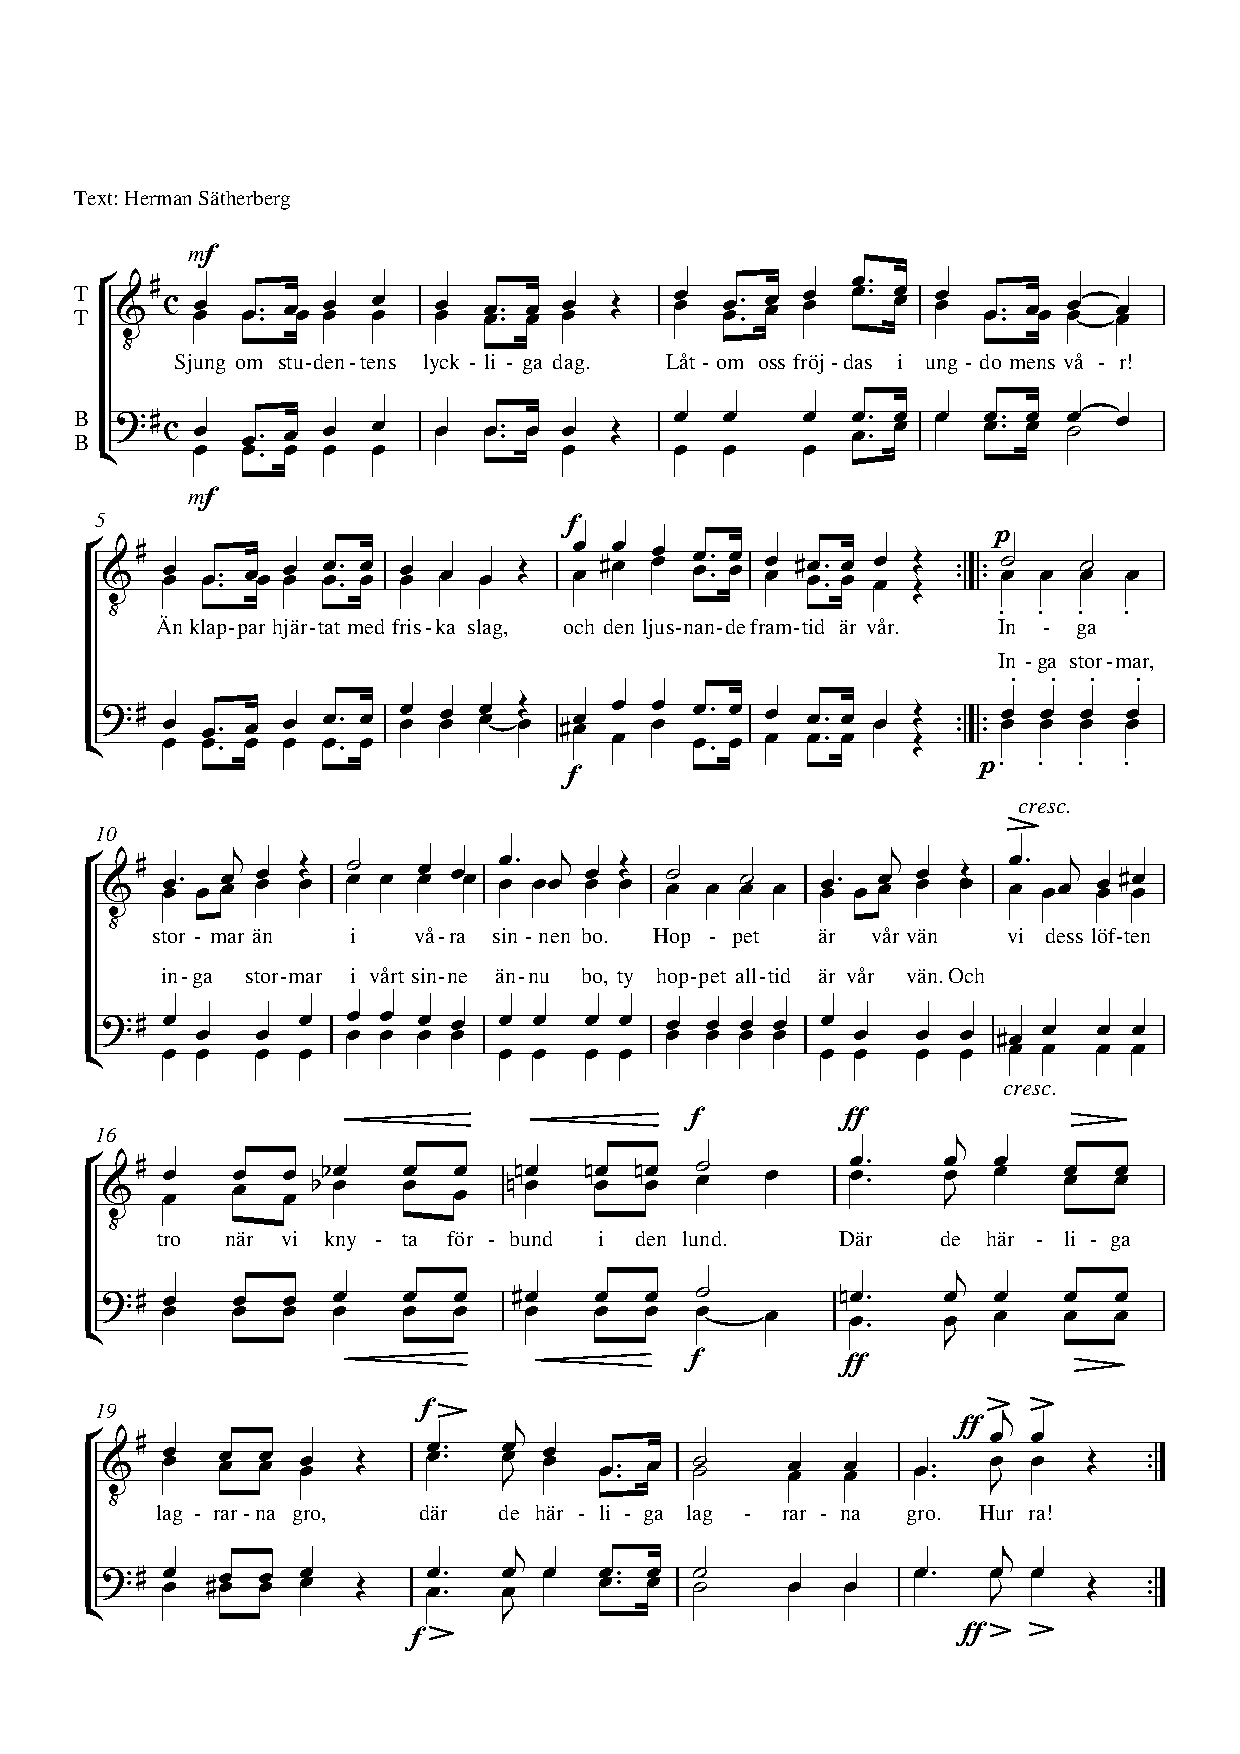
\includegraphics[width=\textwidth]{studentsangen}
\end{figure}

\nysida{16}{12}
\setlength{\oddsidemargin}{-0.67in}
\begin{center}
\Large$\omega\infty$. O gamla klang och jubeltid
\end{center}
\vspace{-40pt}
\begin{figure}[!h]
\centering
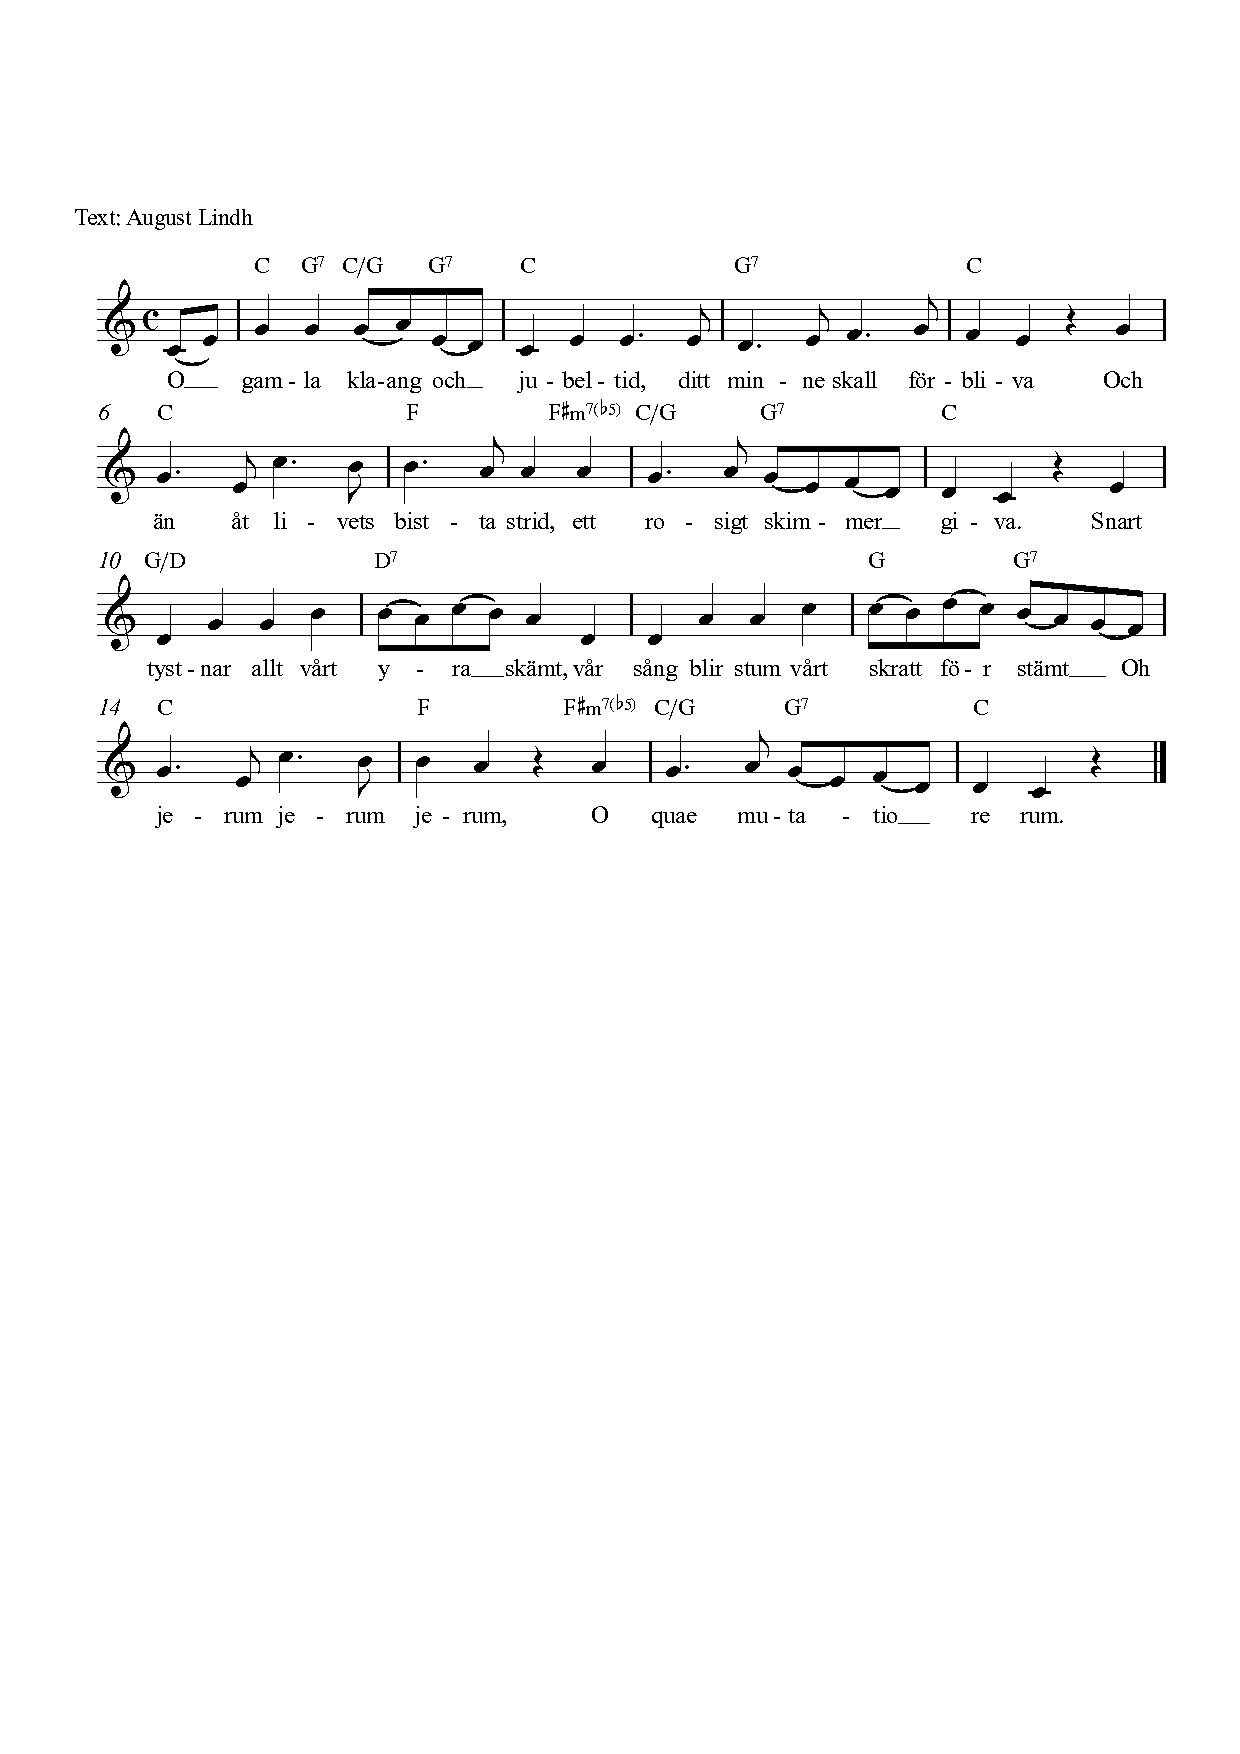
\includegraphics[width=\textwidth]{ogamlaklang}
\end{figure}
\end{document}